\documentclass[11pt]{article}
\RequirePackage{fullpage}
\RequirePackage[font=small,labelfont=bf]{caption}
\RequirePackage{amsmath,amssymb,amsthm}
\RequirePackage{mathtools}
\RequirePackage{graphicx}
\RequirePackage[normalem]{ulem}
\RequirePackage[hidelinks]{hyperref}
\RequirePackage{subcaption}
\RequirePackage{authblk}
\RequirePackage{bm}
\RequirePackage{bbm}
\RequirePackage{tikz}

% line numbers:
\RequirePackage{lineno}
%\modulolinenumbers[5]
\definecolor{linenogray}{gray}{0.75}
\renewcommand\linenumberfont{\normalfont\tiny\sffamily\color{linenogray}}

% spacing
\RequirePackage{setspace}
%\doublespacing
 
% \RequirePackage[osf]{mathpazo}
\RequirePackage[bibstyle=authoryear,citestyle=authoryear-comp,
                date=year,
                maxbibnames=9,maxnames=5,maxcitenames=2,
                backend=biber,uniquelist=false,uniquename=false,
                % style=apa,
                sorting=nyt,
                hyperref=true]{biblatex}
\RequirePackage[colorinlistoftodos]{todonotes}  %disable
\RequirePackage{color}
\RequirePackage{nicefrac}

\newcommand{\gc}[1]{{\it \color{red} #1 } }
\newcommand{\vb}[1]{{\it \color{blue} #1}}
\newcommand{\vbout}[1]{{\it \color{blue} \sout{#1}}}

% a /nonumber you can turn on/off
\newcommand{\nnn}{\nonumber}
%\newcommand{\nnn}{}


\newcommand{\graham}[1]{\todo[size=\scriptsize, color=red!50]{#1}}
\newcommand{\vince}[1]{\todo[size=\scriptsize, color=blue!50]{#1}}

\renewcommand{\P}{\mathbb{P}}
\newcommand{\E}{\mathbb{E}}
\newcommand{\V}{\text{V}}
\newcommand{\cf}{\emph{cf.} }
\DeclareMathOperator{\var}{Var}
\DeclareMathOperator{\cov}{Cov}
\DeclareMathOperator{\flt}{\mathrm{flat}}
\DeclareMathOperator{\T}{{\mathrm{T}}}
\newcommand{\vect}[1]{\mathbf{#1}}
\newcommand{\nssh}{SSH_n}

\newcommand{\chapquote}[2]{\begin{quotation} \textit{#1} \end{quotation} \begin{flushright} - #2\end{flushright} }

\addbibresource{biblio.bib}


% TODO
% - generate figures and write about them
% - Figure 2 has some overplotting issues.

\title{}


\author[$\ast$,$\dag$,$1$]{Vince Buffalo}
\author[$\dag$]{Graham Coop}
\affil[$\ast$]{\footnotesize Population Biology Graduate Group}
\affil[$\dag$]{\footnotesize Center for Population Biology, Department of Evolution and Ecology, University of California, Davis, CA 95616}
\affil[$1$]{\footnotesize Email for correspondence: \href{mailto:vsbuffalo@ucdavis.edu}{vsbuffalo@ucdavis.edu}}

\begin{document}
\maketitle

\section{Introduction}

\section{Results}


% We measure two types of covariances between allele frequency caused by
% selection: temporal autocovariances, and across-replicate covariances. First,
% positive temporal autocovariance in a neutral allele frequency's trajectory
% occurs when the allele becomes associated with a high or low fitness
% chromosomal background, and this association persists through the generations
% due to linkage disequilibrium. As long as the direction of selection remains
% constant, the fitness background is predictive of the direction in the neutral
% allele's frequency changes, creating positive covariance. Even though these
% magnitude of frequency changes at each site may be subtle, as they would be
% under polygenic selection, cumulatively these perturb neighboring sites in a
% predictable manner and build up temporal autocovariance which acts as a
% genome-wide signal of linked selection. Second, if evolution occurs in
% replicate populations undergoing convergent selection pressure, neutral sites
% linked to fitness backgrounds shared across replicates are expected to change
% in the same direction. This creates across-replicate covariance, which is a
% measure of the extent to which convergent selection pressures across replicate
% populations cause similar allele frequency changes. Finally, it is important to
% note that under the null model where the fitness differences between
% individuals are entirely random and non-heritable (e.g. when selection is not
% acting), both forms of covariances are expected to be zero. 

\begin{center}
  \begin{tabular}{l c c c c c c}
    Study & Species & Selection & Replicates & Pop. Size & Gens. & Timepoints \\ 
  \hline
    \textcite{Kelly2019-dc}  & \emph{D. simulans} & lab & 3 & $\sim$1100 & 14 & 2 \\ \hline
    \textcite{Barghi2019-qy} & \emph{D. simulans} & lab & 10 & $\sim$1000 & 60 & 10 \\ \hline
    \textcite{Castro2019-uk} & \emph{M. musculus} & \begin{tabular}{c}tibiae length\\control\end{tabular} & \begin{tabular}{c}2\\1\end{tabular} &\begin{tabular}{c}32\\28\end{tabular}  & 20 & 2 \\
 \hline
\end{tabular}
\end{center}

We first analyzed \textcite{Barghi2019-qy}, an evolve-and-resequence study with
ten replicate populations exposed to a high temperature lab environment and
evolved for 60 generations, and sequenced every ten generations. Using the
seven timepoints and ten replicate populations, we estimated a bias-corrected
genome-wide $6 \times 6$ temporal covariance matrix (a timepoint is lost in
calculating all adjacent allele frequency changes). This temporal covariance
matrix contains 


$60 \times 60$ temporal-replicate variance-covariance matrix (see XXX for
details). 


Since each replicate population was sequenced every ten generations,
the timepoints $t_0 = 0$ generations, $t_1 = 10$ generations, $t_2 = 20$
generations, etc., lead to observed allele frequency changes across ten
generation blocks, $\Delta p_{t_0}, \Delta p_{t_1}, \ldots, \Delta p_{t_6}$.
Consequently, the ten temporal covariance matrices for each of the ten
replicate populations have off-diagonal elements of the form $\cov(\Delta
p_{t_0}, \Delta p_{t_1}) = \cov(p_{t_1} - p_{t_0}, p_{t_2} - p_{t_1}) =
\sum_{i=0}^{10} \sum_{j=10}^{20} \cov(\Delta p_i, \Delta p_j)$. Each diagonal
element has the form $\var(\Delta p_{t_0}) = \sum_{i=0}^{t_0} \var(\Delta
p_{i}) + \sum_{i \ne j}^{t_0} \cov(\Delta p_{i}, \Delta p_{j})$, and is thus a
combination of the effects of drift and selection, as both the variance in
allele frequency changes and cumulative temporal autocovariances terms increase
the variance in allele frequency. With sampling each generation, one could more
accurately partition the total variance in allele frequency change
\parencite{Buffalo2019-io}; while we cannot directly estimate the contribution
of linked selection to the variance in allele frequency change here, the
presence of a positive observed covariance between allele frequency change can
only be caused linked selection. Overall, we expect observed temporal
covariances between timepoints to be weak, some fraction of the additive
genetic variance and linkage disequilibrium that creates temporal
autocovariance decays in the ten generations between sequencing.

\begin{figure}[!ht]
  \centering
  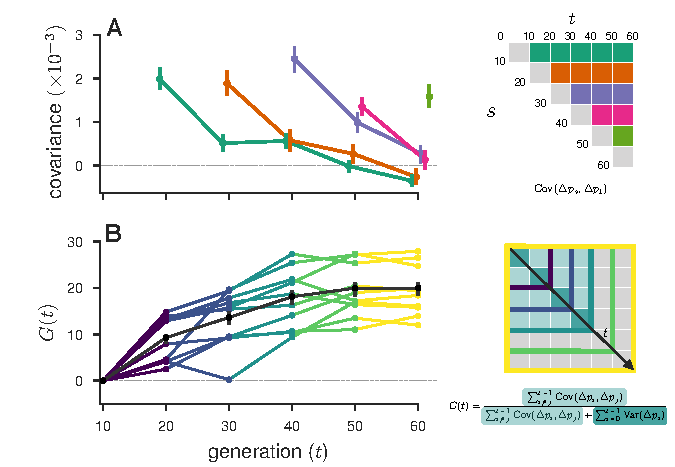
\includegraphics[width=\textwidth]{figures/figure-1.pdf}

  \caption{A: Temporal covariance, averaged across all ten replicate
    populations, through time from the \textcite{Barghi2019-qy} study. Each
    line depicts the temporal covariance $\cov(\Delta p_s, \Delta p_t)$ from
    some reference generation $s$ to a later time $t$ which varies along the
    x-axis; each line corresponds to a row of the upper-triangle of the
    temporal covariance matrix with the same color (upper right). The ranges
    around each point are $95\%$ block-bootstrap confidence intervals. B: The
    proportion of the total variance in allele frequency change explained by
    linked selection, $G(t)$, as it varies through time $t$ along the x-axis.
    The black line is the $G(t)$ averaged across replicates, with the $95\%$
    block-bootstrap confidence interval. The other lines are the $G(t)$ for
    each individual replicate, with colors indicating what subset of the
    temporal-covariance matrix to the right is being included in the
  calculation of $G(t)$.}

  \label{fig:figure-1}
\end{figure}


Averaging across replicate populations, we find positive temporal covariances
across time that are statistically significant (p < XXX) consistent with linked
selection acting to affect allele frequency changes over very short time
periods. We visualize these covariances in Figure \label{figure-1} (A), which
depicts the temporal covariances through time, for each of the five rows
covariance matrix.  Each row represents the temporal covariance $\cov(\Delta
p_s, \Delta p_t)$, between some initial reference generation $s$ (the row of
the matrix), and some later timepoint $t$ (the column of the matrix). For each
row, the covariances at first are positive, and then decay towards zero as
expected when directional selection affects linked variants' frequency
trajectories until ultimately linkage disequilibrium and additive genetic
variance for decay \parencite{Buffalo2019-io}. Note that per replicate, the
signal is a bit noisier; see Supplementary Figures XXX.

While the presence of positive temporal covariances is consistent with linked
selection affecting allele frequencies over time, this measure not easily
interpretable. Additionally, we can quantify the impact of linked selection on
allele frequency change as the ratio of total covariance in allele frequency
change to the total variance in allele frequency change. Since the total
variation in allele frequency change can be decomposed into variance and
covariance components, $\var(p_t - p_0) = \sum_{i \ne j} \cov(\Delta p_i,
\Delta p_j) / \var(p_t - p_0)$, and the covariances are zero when drift acts
alone, this is a lower bound on how much of the variance in allele frequency
change is caused by linked selection \parencite{Buffalo2019-io}. We call this
measure $G(t)$, which is the total effect of linked selection between the
initial generation $0$ and some later generation $t$, which can be varied to
see how this quantity grows through time. As with the temporal covariances, the
study design of \textcite{Barghi2019} leads our measure $G(t)$ to be even more
conservative, since the temporal covariances with each ten-generation block
between sequenced timepoints are not directly observable, and are not included
in the numerator of $G(t)$. Still, we find a remarkably strong signal that
greater than $20\%$ of total variation in allele frequency change over 60
generations is directly the result of linked selection.

% NOTE in supp. material why the average replicate G(t) looks lower than
% replicates.

The replicate design of \textcite{Barghi2019-qy} also allows us to quantify
another covariance: the covariance in allele frequency change between replicate
populations experiencing convergent selection pressure. These between-replicate
covariances are created in the same way as temporal covariances are: neutral
alleles linked to a particular fitness background experience are expected to
have allele frequency changes in the same direction if the selection pressures
are similar. We measure this through a statistic similar to a correlation,
which we call the convergent correlation; this is the ratio of average
between-replicate covariance across all pairs to the average standard deviation
across all pairs of replicates, 

\begin{align}
  \label{eq:conv-corr}
  \mathrm{cor}(\Delta p_s, \Delta p_t) = \frac{\E_{A\ne B} \left( \cov(\Delta p_{s,A}, \Delta p_{t,B}) \right)}{\E_{A\ne B} \left( \sqrt{\var(\Delta p_{s,A}) \var(\Delta p_{t,B})} \right)}
\end{align}
%
where $A$ and $B$ here are two replicate labels.

We've calculated the convergent correlation for all rows of the replicate
covariance matrices, which unlike temporal covariance matrices have diagonal
elements that are also covariances (e.g. $\cov(\Delta p_{t,A}, \Delta
p_{t,B})$). Like temporal covariances, we visualize these through time (Figure
\ref{fig:figure-2} A), with each line representing the convergent correlation
from a particular reference generation $s$ as it varies with $t$ (shown on the
x-axis). In other words, each of the colored lines corresponds to the like
colored row of the convergence correlation matrix (upper left in Figure
\ref{fig:figure-2} A). We find these decay very quickly, from an initial
convergence correlation coefficient of about 0.1 (block bootstrap confidence
intervals XXX; see the note in Supplementary Material XXX why these are so
narrow), to around 0.01 within 20 generations.

A benefit of between-replicate covariances is unlike temporal covariances,
these can be calculated with only two sequenced timepoints and a replicated
study design. This allowed allowed us to assess the impact of linked selection
in driving convergent patterns of allele frequency change across replicate
populations in two other studies. First, we reanalyzed the selection experiment
of \textcite{Kelly2019-dc}, which evolved three replicate populations of
\emph{Drosophila simulans} for 14 generations in a novel laboratory
environment. Since each replicate was exposed to the same selection pressure
and share linkage disequilibria common to the original natural founding
population, we expected each of the three replicate populations to have
positive between-replicate covariances. We find all three pairwise
between-replicate covariances are positive and statistical significant (p <
XXX, estimated via block bootstrap). We estimate the convergent correlation
coefficient across these replicates as 0.36 ($95\%$ block-bootstrap confidence
interval $[0.31, 0.40]$).

Second, we reanalyzed the Longshanks selection experiment, which selected for
longer tibiae length relative to body size in mice, leading to a response of
selection of about 5 standard deviations over the course of twenty generations
\parencite{Castro2019-uk}. This study includes two independent selection lines,
Longshanks 1 and 2 (LS1 and LS2), and an unselected control line (Ctrl).
Consequently, this selection experiment offers a useful control to test our
between-replicate covariances: we expect to see positive between-replicate
covariance in the comparison between the two Longshanks selection lines, but
not between the two pairwise comparisons between the control line and the two
Longshanks lines. We find that this is the case (Figure \ref{fig:figure-2} C),
with the two Longshanks comparisons to the control line not being significantly
different from zero, while the comparison between the two Longshanks line is
statistically significantly different from zero (CIs XXX).

Paragraph about large effect loci.

\begin{figure}[!ht]
  \centering
  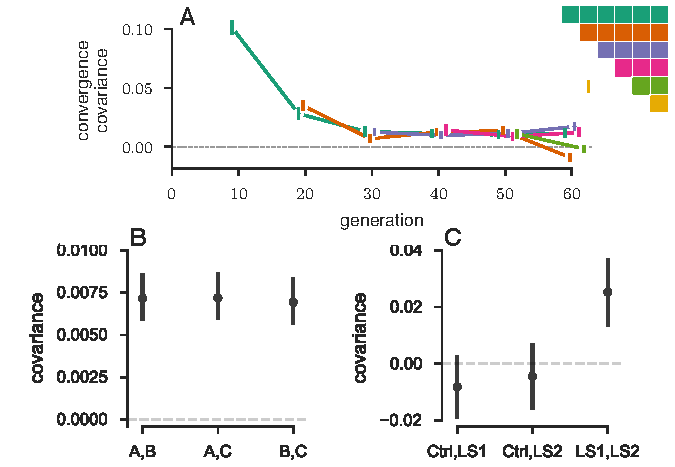
\includegraphics[width=\textwidth]{figures/figure-2.pdf}

  \caption{A: The convergence correlation, averaged across replicate pairs,
    through time. Each line represents the convergence correlation
    $\mathrm{cor}(\Delta p_{s}, \Delta p_{s})$ from a starting reference
    generation $s$ to a later time $t$, which varies along the x-axis; each
  line corresponds to a row of the temporal convergence correlation matrix
depicted to the right.}

  \label{fig:figure-2}
\end{figure}

Finally, we observed that in the longest run evolve-and-resequence study we
analyzed \parencite{Barghi2019-qy}, some temporal covariances appeared to
become negative at future timepoints (see the first two rows in Figure
\ref{fig:figure-1} A). This could be caused by advantageous fitness backgrounds
later becoming disadvantageous, either due to frequency-dependent selection,
recombination breaking up coupled beneficial and deleterious alleles, or an
environmental change in the direction of selection. However, the signal of a
change in the direction of selection localized to a particular region of the
genome may be washed out when we calculate genome-wide temporal covariances.
Averaging over such large numbers of loci is necessary to detect a signal of
covariance in allele frequency changes when both drift (inflated in
evolve-and-sequence studies which use small population sizes) and sampling
variance can create spurious covariances. To address this limitation, we
calculated temporal covariances over 100kb genomic windows, with on average XXX
loci per window. While the covariance of each tile is noisy, we can analyze the
genome-wide distribution of tile covariances for changes through time. We would
like to compare the distribution of these tile covariances to a neutral
expectation, but using a theoretic neutral null distribution would be
inappropriate given complex dependencies across the genome due to linkage
disequilibria (which can occur over long physical distances in E\&R and
selection studies, \cite{Nuzhdin2013-gf,Baldwin-Brown2014-cl}). 

Instead, we have developed a permutation-based procedure that constructs a null
distribution of the genome-wide covariances as they would look if only neutral
genetic drift was acting. We do this by randomly flipping the signs of the
allele frequency changes per-genomic window 1,000 times, which acts to destroy
the systematic covariances created by linked selection but creates a sampling
distribution of the covariances spuriously created by neutral genetic drift.
This empirical neutral null distribution is conservative in the sense that the
variances of the covariances are wider than expected under drift alone, since
drift also acts to inflate the magnitude of allele frequency change. By
flipping the sign at the block-level, we preserve the complex dependencies
between adjacent loci created by linkage disequilibrium; see Supplementary
Material Section \ref{supp:empirical-null} for more details on this approach.

Using the \textcite{Barghi2019-qy} study's data, we used the empirical neutral
null to investigate whether there was a general trend for the temporal
covariance $\cov(\Delta p_t, \Delta p_{t+k})$ to be positive for small $k$ (as
expected under selection), but then become systematically negative for larger
$k$ (as would occur under evolutionary processes that reverse the fitness of
regions across the genome). Such a change in the fitness direction of
haplotypes would not be discernible from genome-wide covariances like those in
Figure \ref{fig:figure-1}. We find (Figure \ref{fig:figure-3} A and B), pooling
across all replicates (see Supplementary Figure
\ref{suppfig:barghi-offset-replicate-panels} for individuals replicates), that
windowed temporal covariances between close timepoints are skewed positive (a
heavy right tail), while between more distant timepoints these windowed
temporal covariances tend to shift to become more negative (a heavy left tail).


\begin{figure}[!ht]
  \centering
  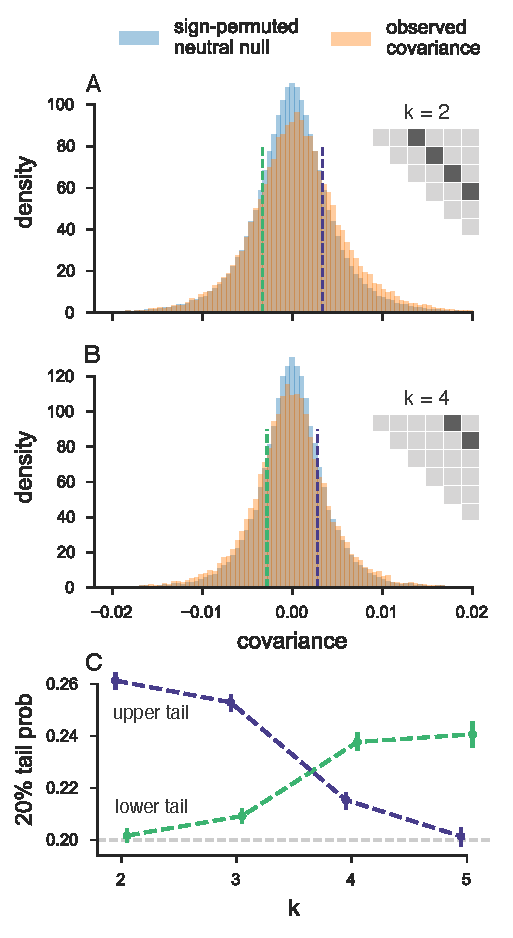
\includegraphics[]{figures/figure-3.pdf}

  \caption{A, B: The distribution of temporal covariances calculated in 100kb
    genomic windows from the \textcite{Barghi2019-qy} study, plotted alongside
    an empirical neutral null distribution created by recalculating the
    windowed covariances on sign permuting the allele frequency changes. In
    subfigure A, windowed covariances $\cov(\Delta p_t, \Delta p_{t+k})$ are
    separated by $k=2 \times 10$ generations and in subfigure B the covariances
    are separated by $k=4 \times 10$ generations; each $k$ is an off-diagonal
    from the variance diagonal of the temporal covariance matrix (see cartoon
    of upper-triangle of covariance matrix in subfigures A and B, where the red
    diagonal is the variance, and the dark gray indicates which off-diagonal of
    the covariance matrix is plotted in the histograms). C: The lower and upper
    tail probabilities of the observed windowed covariances, at 20\% and 80\%
    quintiles of the empirical neutral null distribution, for varying time
    between allele frequency changes (i.e. which off-diagonal $k$). The
    confidence intervals are  $95\%$ block-bootstrap confidence interval, and the
    light gray dashed line indicates the 20\% tail probability expected under the
    neutral null.}
  
    \label{fig:figure-3} 
\end{figure}


% \begin{figure}[!ht]
%   \centering
%   \includegraphics[width=\textwidth]{}
%   \caption{}
%   \label{}
% \end{figure}

\section{Acknowledgments} 

Doc Edge.


\section{Appendix}

\section{Estimator Bias Correction}
\subsection{Correcting variance bias with a single depth sampling process}
\label{supp:depth-var-corr}

Following \textcite{Waples1989-sj}, we have that that the variance in the
initial generation, which is entirely due to the binomial sampling process, is
$\var(p_0) = \nicefrac{p_0(1-p_0)}{d_0}$ where $d_0$ is the number of binomial
draws (e.g. read depth). At a later timepoint, the variance in allele frequency
is a result of both the binomial sampling process at time $t$ and the
evolutionary process.

Using the law of total variation, 

\begin{align}
  \var(\widetilde{p_t}) &= \E(\var(\widetilde{p_t} | p_t)) + \var(\E(\widetilde{p_t}|p_t)) \\
                        &= \underbrace{\frac{p_t(1-p_t)}{d_t}}_\text{generation $t$ sampling noise} + \underbrace{\var(p_t)}_\text{variance due to evolutionary process}
  %\frac{\var(\widetilde{p_t})}{p_0(1-p_0)} &= \frac{p_t(1-p_t)}{p_0(1-p_0) d_t} + 1 - \left( 1-\frac{1}{2N}\right)^t.
  %\frac{\var(\widetilde{p_t})}{p_0(1-p_0)} &= \frac{p_t(1-p_t)}{p_0(1-p_0) d_t} + \frac{t}{2N} + O\left((2 N)^{-2}\right).
\end{align}

Under a drift-only process, $\var(p_t) = p_0(1-p_0)\left[1- \left(1 -
\frac{1}{2N}\right)^t\right]$. However, with heritable variation in fitness, we
need to consider the covariance in allele frequency changes across generations
\parencite{Buffalo2019-io}. We can write

\begin{align}
  V(p_t) &= V\left(p_0 + (p_1 - p_0) + (p_2 - p_1) + \ldots + (p_t - p_{t-1}) \right) \\
         &= V\left(p_0 + \Delta p_0 + \Delta p_1 + \ldots + \Delta p_{t-1} \right) \\
         &= V(p_0) + \sum_{i=0}^{t-1} \cov(p_0, \Delta p_i) + \sum_{i=0}^{t-1} \var(\Delta p_i) + \sum_{0 \le i < j}^{t-1} \cov(\Delta p_i, \Delta p_j).
\end{align}
%

Each allele frequency change is equally like to be positive as it is to be
negative; thus by symmetry this second term is zero. Additionally $V(p_0) = 0$,
as we treat $p_0$ as a fixed initial frequency. We can write, 

\begin{align}
  V(p_t) &= \sum_{i=0}^{t-1} \var(\Delta p_i) + \sum_{0 \le i < j}^{t-1} \cov(\Delta p_i, \Delta p_j).
\end{align}

The second term, the cumulative impact of variance in allele frequency change
can be partitioned into heritable fitness and drift components
\parencite{Santiago1995-hx,Buffalo2019-io}

\begin{align}
  V(p_t) &= \sum_{i=0}^{t-1} \var(\Delta_{_D} p_i) + \sum_{i=0}^{t-1} \var(\Delta_{_H} p_i) + \sum_{0 \le i < j}^{t-1} \cov(\Delta p_i, \Delta p_j).
\end{align}

where $\Delta_{_H} p_t$ and $\Delta_{_D} p_t$ indicate the allele frequency
change due to heritable fitness variation and drift respectively. Then, sum of
drift variances in allele frequency change is

\begin{align}
  \sum_{i=0}^{t-1} \var(\Delta_{_D} p_i) = \sum_{i=0}^{t-1} \frac{p_i(1-p_i)}{2N}
\end{align}

replacing the heterozygosity in generation $i$ with its expectation, we have

\begin{align}
  \sum_{i=0}^{t-1} \var(\Delta_{_D} p_i) &= p_0(1-p_0) \sum_{i=0}^{t-1} \frac{1}{2N} \left(1-\frac{1}{2N}\right)^i \\
                                         &= p_0(1-p_0) \left[1 - \left(1-\frac{1}{2N}\right)^t \right]
\end{align}

which is the usual variance in allele frequency change due to drift.  Then, the
total allele frequency change from generations $0$ to $t$ is
$\var(\widetilde{p}_t - \widetilde{p}_0) = \var(\widetilde{p}_t) +
\var(\widetilde{p}_0) - 2 \cov(\widetilde{p}_t, \widetilde{p}_0)$, where the
covariance depends on the nature of the sampling plan (see \cite{Nei1981-oy,
Waples1989-sj}). In the case where there is heritable variation for fitness,
and using the fact that $\cov(\widetilde{p}_t, \widetilde{p}_0) =
\nicefrac{p_0(1-p_0)}{2N}$ for Plan I sampling procedures
\parencite{Waples1989-sj}, we write,

\begin{align}
  \var(\widetilde{p}_t - \widetilde{p}_0) &= \var(\widetilde{p}_t) + \var(\widetilde{p}_0) - 2 C \cov(\widetilde{p}_t, \widetilde{p}_0) \\
                                          &= \frac{p_t(1-p_t)}{d_t}  + \frac{p_0(1-p_0)}{d_0} + p_0(1-p_0) \left[1 - \left(1-\frac{1}{2N}\right)^t \right] + \\ & \;\;\;\;\;\;
                                               \sum_{i=0}^{t-1} \var(\Delta_{_H} p_i)  + \sum_{0 \le i < j}^{t-1} \cov(\Delta p_i, \Delta p_j) - \frac{C p_0(1-p_0)}{2N} \\
  \frac{\var(\widetilde{p}_t - \widetilde{p}_0)}{p_0(1-p_0)} &= 1 + \frac{p_t(1-p_t)}{p_0(1-p_0)d_t}  + \frac{1}{d_0} - \left(1-\frac{1}{2N}\right)^t + \\ & \;\;\;\;\;\;
  \sum_{i=0}^{t-1} \frac{\var(\Delta_{_H} p_i)}{p_0(1-p_0)}  + \sum_{0 \le i < j}^{t-1} \frac{\cov(\Delta p_i, \Delta p_j)}{p_0(1-p_0)} - \frac{C}{N}
\end{align}

where $C = 1$ if Plan I is used, and $C=0$ if Plan II is used (see
\cite{Waples1989-sj}, p. 380 and Figure 1 for a description of these sampling
procedures). We move terms creating a corrected estimator for the population
variance in allele frequency change, and replace all population heterozygosity
terms with the unbiased sample estimators, e.g. $\frac{d_t}{d_t-1}
\widetilde{p}_t (1- \widetilde{p}_t)$,

\begin{align}
  \label{supp:eqn-depth-only-correction}
  \frac{d_0-1}{d_0} \frac{\var(\widetilde{p}_1 - \widetilde{p}_0)}{\widetilde{p}_0(1-\widetilde{p}_0)} - \frac{(d_0-1)}{d_0 (d_1 - 1)} \frac{\widetilde{p}_1(1-\widetilde{p}_1)}{\widetilde{p}_0(1-\widetilde{p}_0)} - \frac{1}{d_0} + \frac{C}{N}  &= \frac{\var(\Delta_{_H} p_0)}{p_0(1-p_0)} + \frac{1}{2N} 
\end{align}

\subsection{Correcting variance bias with individual and depth sampling processes}
\label{supp:ind-depth-var-corr}

Here, we extend the sampling bias correction described above to handle two
binomial sampling processes: one as individuals are binomially sampled from the
population, and another as reads are binomially sampled during sequencing.
(see also \cite{Jonas2016-ia}). Let $X_t \sim \text{Binom}(n_t, p_t)$ where
$X_t$ is the count of alleles and $n_t$ is the number of diploids sampled at
time $t$. Then, these individuals are sequenced at a depth of $d_t$, and $Y_t
\sim \text{Binom}(d_t, \nicefrac{X_t}{n_t})$ reads have the tracked allele. We
let $\widetilde{p_t} = \nicefrac{Y_t}{d_t}$ be the observed sample allele
frequency. Then, the sampling noise is 

\begin{align}
  \var(\widetilde{p_t}|p_t) &= \E(\var(\widetilde{p_t} | X_t)) + \var(\E(\widetilde{p_t} | X_t)) \\
                            &= p_t(1-p_t) \left(\frac{1}{n_t} + \frac{1}{d_t} - \frac{1}{n_t d_t} \right)
\end{align}


\begin{align}
  \var(\widetilde{p}_t - \widetilde{p}_0) &= 
  p_t(1-p_t) \left(\frac{1}{n_t} + \frac{1}{d_t} - \frac{1}{n_t d_t} \right)  
  + p_0(1-p_0) \left( \frac{1}{n_0} + \frac{1}{d_0} - \frac{1}{n_0 d_0}\right)  \\ & \;\;\;\;\;\;
  - \frac{C p_0(1-p_0)}{N} + p_0(1-p_0) \left[1 - \left(1-\frac{1}{2N}\right)^t \right]+ \sum_{i=0}^{t-1} \var(\Delta_{_H} p_i)  \\ & \;\;\;\;\;\; + \sum_{0 \le i < j}^{t-1} \cov(\Delta p_i, \Delta p_j) 
\end{align}

Through the law of total expectation, one can find that an unbiased estimator
of the heterozygosity is 

\begin{align}
  \frac{n_t d_t}{(n_t-1) (d_t-1)} \widetilde{p_t}(1-\widetilde{p_t}).
\end{align}

Replacing this unbiased heterozygosity into our expression above, the total
sample variance is

\begin{align}
  \var(\widetilde{p}_t - \widetilde{p}_0) &= 
  \frac{n_t d_t \widetilde{p}_t(1-\widetilde{p}_t)}{(n_t-1)(d_t-1)} \left(\frac{1}{n_t} + \frac{1}{d_t} - \frac{1}{n_t d_t} \right) + 
 \frac{n_0 d_0 \widetilde{p}_0(1-\widetilde{p}_0)}{(n_0-1)(d_0-1)} \left( \frac{1}{n_0} + \frac{1}{d_0} - \frac{1}{n_0 d_0}\right) + \\ & \nonumber\;\;\;\;\;\;
 \frac{n_0 d_0 \widetilde{p}_0(1-\widetilde{p}_0)}{(n_0-1)(d_0-1)}   \left[1 - \left(1-\frac{1}{2N}\right)^t \right]  - \frac{C}{N}  \frac{n_0 d_0 \widetilde{p}_0(1-\widetilde{p}_0)}{(n_0-1)(d_0-1)} + \\ \nonumber & \;\;\;\;\;\; \sum_{i=0}^{t-1} \var(\Delta_{_H} p_i)  + \sum_{0 \le i < j}^{t-1} \cov(\Delta p_i, \Delta p_j).  \\
                                                                                                                      % &= \widetilde{p}_t(1-\widetilde{p}_t)\frac{d_t + n_t - 1}{(n_t-1)(d_t-1)} + 
 % \widetilde{p}_0(1-\widetilde{p}_0)\frac{d_0 + n_0 - 1}{(n_0-1)(d_0-1)} + \\ & \nonumber\;\;\;\;\;\;
 % \widetilde{p}_0(1-\widetilde{p}_0) \frac{n_0 d_0}{(n_0-1)(d_0-1)}  \left[1 - \left(1-\frac{1}{2N}\right)^t \right] - \frac{C}{N} \widetilde{p}_0(1-\widetilde{p}_0)\frac{n_0 d_0}{(n_0-1)(d_0-1)} 
 % \\ \nonumber & \;\;\;\;\;\; + \sum_{i=0}^{t-1} \var(\Delta_{_H} p_i)  + \sum_{0 \le i < j}^{t-1} \cov(\Delta p_i, \Delta p_j). 
\end{align}

As with equation \eqref{supp:eqn-depth-only-correction}, we can rearrange this
to get a biased-correct estimate of the variance in allele frequency change
between adjacent generations, $\var(\Delta p_t)$. 


\subsection{Covariance Correction}
\label{supp:cov-corr}

We also need to apply a bias correction to the temporal covariances (and
possibly the replicate covariances if the initial sample frequencies are all
shared).

The basic issue is that $\cov(\Delta \widetilde{p}_t, \Delta
\widetilde{p}_{t+1}) = \cov(\widetilde{p}_{t+1} - \widetilde{p}_t,
\widetilde{p}_{t+2} - \widetilde{p}_{t+1})$, and thus shares the sampling noise
of timepoint $t+1$. Thus acts to bias the covariance by subtracting off the
noise variance term of $\var(\widetilde{p}_{t+1})$, so we add that back in.

\subsection{Variance-Covariance Matrix Correction}

Now, we extend the bias corrections for single locus variance and covariance
described in Supplementary Material Sections \ref{supp:depth-var-corr},
\ref{supp:ind-depth-var-corr}, and \ref{supp:cov-corr} to multiple sampled
loci. With frequency collected at $T+1$ timepoints across $R$ replicate
populations at $L$ loci, we have $\mathbf{F}$ of allele frequencies,
$\mathbf{D}$ multidimensional array of sequencing depths, and a $\mathbf{N}$
multidimensional array of the number of individuals sequenced, each of
dimension $R \times (T+1) \times L$.  We calculate the array $\mathbf{\Delta
F}$ which contains the allele frequency changes between adjacent generations,
and has dimension $R \times T \times L$.  The operation
$\flt(\mathbf{\Delta}\mathbf{F})$ flattens this array to a $(R \cdot T) \times
L$ matrix, such that rows are grouped by replicate, e.g. for timepoint $t$,
replicate $r$, and locus $l$ and allele frequencies $p_{t, r}$, for a single
locus the entries are 

% \begin{align}
%   \mathbf{\Delta F} &= 
%                     &\begin{bmatrix} 
%     p_{1, 0, 0} - p_{0, 0, 0} & p_{2, 0, 0} - p_{1, 0, 0} & \ldots & p_{1, 1, 0} - p_{0, 1, 0} & p_{2, 1, 0} - p_{1, 1, 0} & \ldots & p_{T+1, R, 0} - p_{T, R, 0}  \\
%     p_{1, 0, 1} - p_{0, 0, 1} & p_{2, 0, 1} - p_{1, 0, 1} & \ldots & p_{1, 1, 1} - p_{0, 1, 1} & p_{2, 1, 1} - p_{1, 1, 1} & \ldots & p_{T+1, R, 1} - p_{T, R, 1}  \\
%     \vdots & \vdots & \ddots & \vdots & \vdots & \ddots & \vdots  \\
%     p_{1, 0, L} - p_{0, 0, L} & p_{2, 0, L} - p_{1, 0, L} & \ldots & p_{1, 1, L} - p_{0, 1, L} & p_{2, 1, L} - p_{1, 1, L} & \ldots & p_{T+1, R, L} - p_{T, R, L}  \\
%   \end{bmatrix} 
% \end{align}

\begin{align}
    \flt(\mathbf{\Delta F}) &=
                    &\begin{bmatrix} 
    \Delta p_{1, 0, 0} & \Delta p_{2, 0, 0} & \ldots & \Delta p_{1, 1, 0} & \Delta p_{2, 1, 0} & \ldots & \Delta p_{T, R, 0}  \\
    \Delta p_{1, 0, 1} & \Delta p_{2, 0, 1} & \ldots & \Delta p_{1, 1, 1} & \Delta p_{2, 1, 1} & \ldots & \Delta p_{T, R, 1}  \\
    \vdots & \vdots & \ddots & \vdots & \vdots & \ddots & \vdots  \\
    \Delta p_{1, 0, L} & \Delta p_{2, 0, L} & \ldots & \Delta p_{1, 1, L} & \Delta p_{2, 1, L} & \ldots & \Delta p_{T, R, L}  \\
  \end{bmatrix} 
\end{align}

where each $\Delta p_{t, r, l} = p_{t+1, r, l} - p_{t, r, l}$. Then, the sample
temporal-replicate covariance matrix $\mathbf{Q}'$ calculated on
$\flt(\mathbf{\Delta F})$ is a $(R \cdot T) \times (R \cdot T)$ matrix, with
the $R$ temporal-covariance block submatrices along the diagonal, and the
$R(R-1)$ replicate-covariance submatrices matrices in the upper and lower
triangles of the matrix,

\begin{align}
	\mathbf{Q}' &= 
  \begin{bmatrix} 
		\mathbf{Q}_{1,1}' & \mathbf{Q}_{1, 2}' & \ldots & \mathbf{Q}_{1, R}' \\ 
		\mathbf{Q}_{2,1}' & \mathbf{Q}_{2, 2}' & \ldots & \mathbf{Q}_{2, R}' \\ 
		\vdots & \vdots & \ddots & \vdots \\
		\mathbf{Q}_{R,1}' & \mathbf{Q}_{R, 2}' & \ldots & \mathbf{Q}_{R, R}' \\ 
  \end{bmatrix} 
\end{align}
%
where each submatrix $\mathbf{Q}_{i,j}'$ is the $T \times T$ sample covariance
matrix for replicates $i$ and $j$.  

Given the bias of the sample covariance of allele frequency changes, we
calculated an expected bias matrix $\mathbf{B}$, averaging over loci,

\begin{align}
  \mathbf{B} = \frac{1}{L} \sum_{l=1}^L \frac{\mathbf{h}_l}{2} \circ \left( \frac{1}{\mathbf{d}_l} + \frac{1}{2\mathbf{n}_l} + \frac{1}{2\mathbf{d}_l \circ \mathbf{n}_l} \right)
\end{align}
%
where $\circ$ denotes elementwise product, and $\mathbf{h}_l$, $\mathbf{d}_l$,
and $\mathbf{n}_l$, are rows corresponding to locus $l$ of the unbiased
heterozygosity arrays $\mathbf{H}$, depth matrix $\mathbf{D}$, and number of
diploids matrix $\mathbf{N}$. The unbiased $R \times (T+1) \times L$
heterozygosity array can be calculated as  

\begin{align}
  \mathbf{H} = \frac{2 \mathbf{D} \circ \mathbf{N} }{ (\mathbf{D}-1) \circ (\mathbf{N} -1)} \circ \mathbf{F} \circ (1-\mathbf{F})
\end{align}
%
where division here is elementwise. Thus, $\mathbf{B}$ is a $R \times (T+1)$
matrix. As explained in Supplementary Material Section
\ref{supp:ind-depth-var-corr} and \ref{supp:cov-corr}, the temporal variances
and covariances require bias corrections, meaning each temporal covariance
submatrix $\mathbf{Q}_{r,r}$ requires two corrections. For an element
$Q_{r,t,s} = \cov(\Delta p_t, \Delta p_s)$ of the temporal covariance submatrix
for replicate $r$, $\mathbf{Q}_{r,r}$, we apply the following correction

\begin{equation}
	Q_{r,t,s} =  
		\begin{dcases}
			Q_{r,t,s}' - b_{r,t} - b_{r,t+1}, & \text{if  } t = s \\
      Q_{r,t,s}' + b_{r,\max(t,s)}, & \text{if  } |t - s| = 1 \\
		\end{dcases}
\end{equation}

where $b_{r,t}$ is element in row $r$ and column $t$ of $\mathbf{B}$.
Additionally, in some study designs, a single timepoint is shared for the
initial generation across replicates. In this case, the sampling noise is
shared between 



\subsection{Block Bootstrap Procedure}
\label{supp:block-bootstrap}

To infer the uncertainty of covariance, convergence correlation, and $G(t)$
estimates, we used a block bootstrap procedure. This is a version of the
bootstrap that resamples blocks of data points, rather than individual data
points, to infer the uncertainty of an statistic in the presence of unknown
correlation structure between data. With genome-wide data, linkage
disequilibria between sites creates complex and unknown dependencies between
variants. The estimators used in this paper are predominantly ratios, e.g.
temporal-replicate covariance standardized by half the heterozygosity (XXX),
$G(t)$ which is the ratio of covariance to total variance (XXX), and the
convergence correlation (equation \eqref{eq:conv-corr}). In these cases, we can
exploit the linearity of the expectation to make the bootstrap procedure more
computationally efficient, by pre-calculating the statistics of the ratio's
numerator and denominator, $N(\mathbf{x}_i)$ and $D(\mathbf{x}_i)$, on the data
$\mathbf{x}_i$ for all blocks $i \in \{1, 2, \ldots, W\}$ in the genome. Then
we draw $W$ bootstrap samples with replacement, and compute the estimate for
bootstrap sample $b$ with an average weighted by the number of loci in all
sampled blocks, 

\begin{align}
  \tilde{\theta}_b = \sum_{i=1}^W w_i \frac{N(\mathbf{x}_i)}{D(\mathbf{x}_i)}
\end{align}
%
Note that computing the ratio of averages rather than the average of a ratio is
a practice common for population genetic statistics like $F_{ST}$
\parencite{Bhatia2013-zy}. With these $B$ bootstrap estimates, we calculate the
$\nicefrac{\alpha}{2}$ and $1-\nicefrac{\alpha}{2}$ quantiles, which we use to
estimate the $1-\alpha = 95\%$ pivot confidence intervals (p. 33
\cite{Wasserman2006-jl}, p. 194 \cite{Davison2013-oy}) throughout the paper,

\begin{align}
  C_\alpha = \left(2 \widehat{\theta} - q_{1-\nicefrac{\alpha}{2}}, 2 \widehat{\theta} - q_{\nicefrac{\alpha}{2}} \right).
\end{align}
%
where $\widehat{\theta}$ is the estimate, and $q_x$ is bootstrap quantile for
probability $x$.

\subsection{The Empirical Neutral Null Windowed Covariance Distribution}
\label{supp:empirical-null}




\section{Supplementary Figures}

\subsection{Bias Correction for \textcite{Barghi2019-qy}}

We have investigated the effectiveness of our correction on real data by
exploiting the relationship between sampling depth and the magnitude of the
variance and covariance biases, and comparing the observed variances and
covariances before and after correction. We plot the variance and covariance
(between adjacent timepoints) before and after the bias correction against the
average sample depth in 100kb genomic windows in Figure
\ref{suppfig:barghi-correction}. Overall, we find the correction strongly

\begin{figure}[!ht]
  \centering
  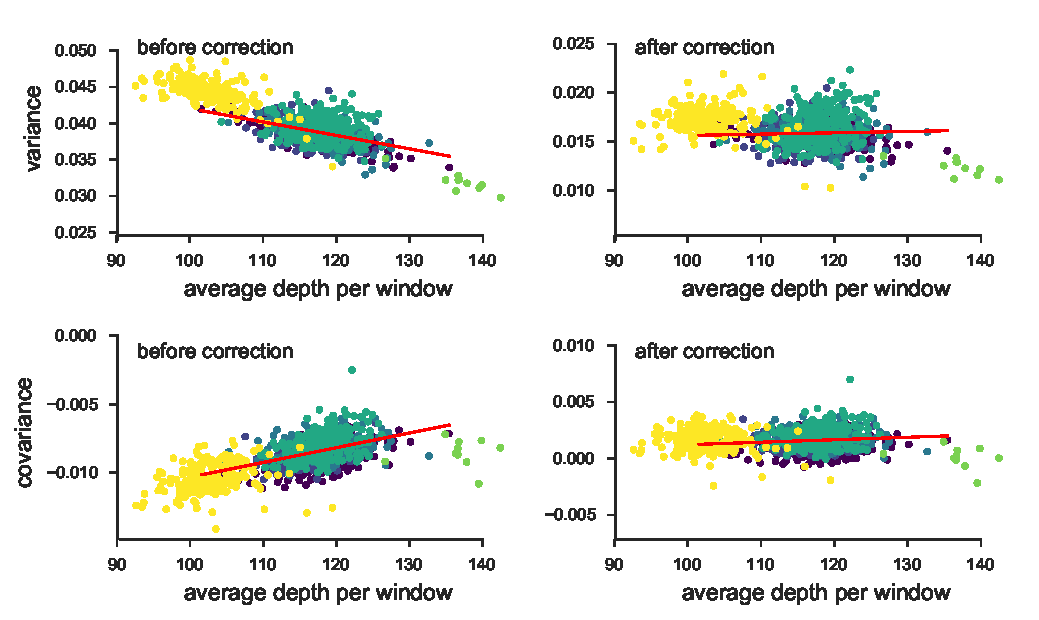
\includegraphics[]{figures/barghi-correction-plot.pdf}

  \caption{The variance and covariances calculated in 100kb genomic windows
    plotted against average depth in a window before and after bias correction.
    Each panel has a least-squares estimate between the variance and
    covariance, and the average depth. Overall, the bias correction corrects
    sampling bias in both the variance and covariance such that the
    relationship with depth is constant. Colors indicate the different
    chromosomes of \emph{D. simulans}; we have excluded the X chromosome
    (yellow points) and chromosome 4 points (green points to far right) from
    the regression due to large differences in average coverage.}

  \label{suppfig:barghi-correction}
\end{figure}

\subsection{\textcite{Barghi2019-qy} Empirical Null and Windowed Covariance Distributions}

\begin{figure}[!ht]
  \centering
  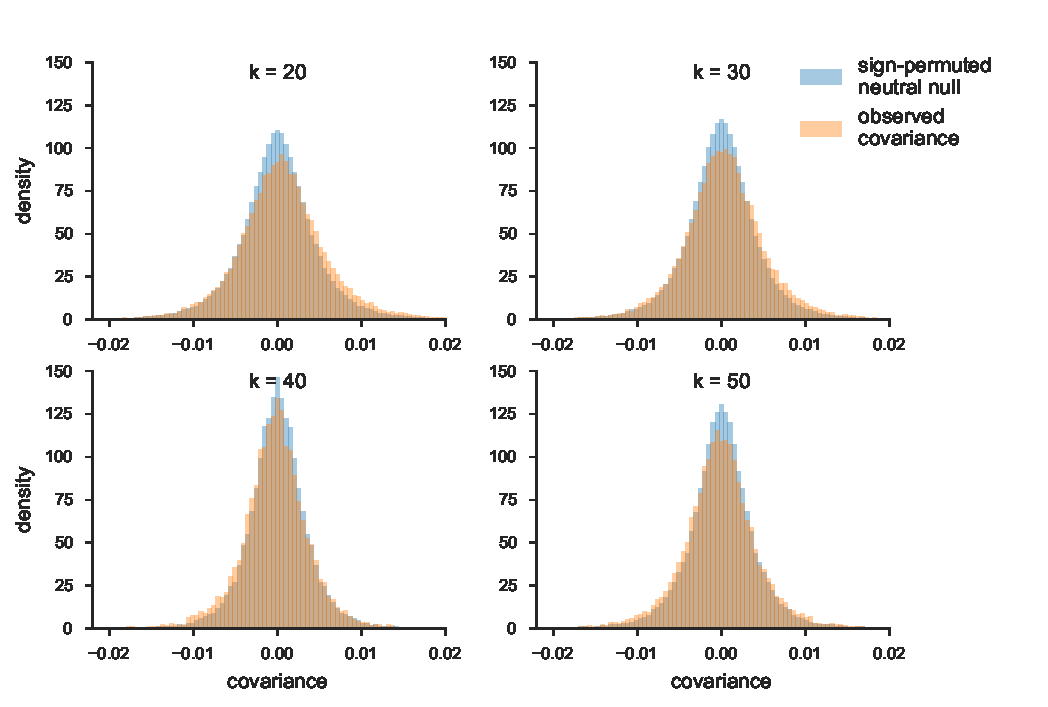
\includegraphics[]{figures/barghi-offset-panels.pdf}

  \caption{The distribution of temporal covariances calculated across 100kb
    genomic windows from \textcite{Barghi2019-qy}'s study (orange) and the
    block sign permuted empirical neutral null distribution of the windowed
    covariances (blue). Each panel shows these windowed covariances and the
    empirical null distribution for covariances $\cov(\Delta p_t, \Delta p_{t+k})$,
  $k$ is the number of generations between allele frequency changes.}
  \label{suppfig:barghi-empnull-tilecovs}
\end{figure}


\begin{figure}[!ht]
  \centering
  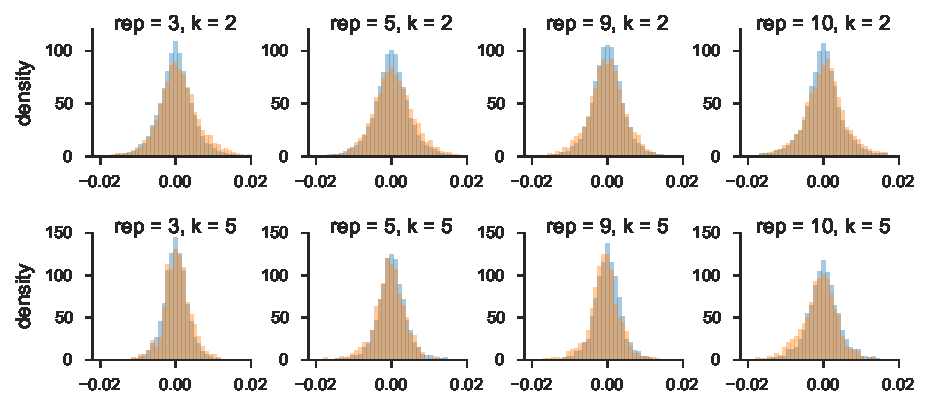
\includegraphics[]{figures/barghi-offset-replicate-panels.pdf}

  \caption{The distribution of windowed temporal covariances alongside the
    empirical neutral null for five randomly sampled replicates (columns), for
    $k=2$ (first row) and $k=5$ (second row). The main figure of the paper
    pools all replicate window and empirical neutral null covariances; we show
    here the windowed temporal covariances tend to shift from being positive (a
    heavier right tail) to become more negative (a heavier left tail) through
    time within particular replicates.}
  
  \label{suppfig:barghi-offset-replicate-panels}
\end{figure}



\subsection{\textcite{Barghi2019-qy} Tail Probabilities for Windowed Covariances Distributions}

\begin{figure}[!ht]
  \centering
  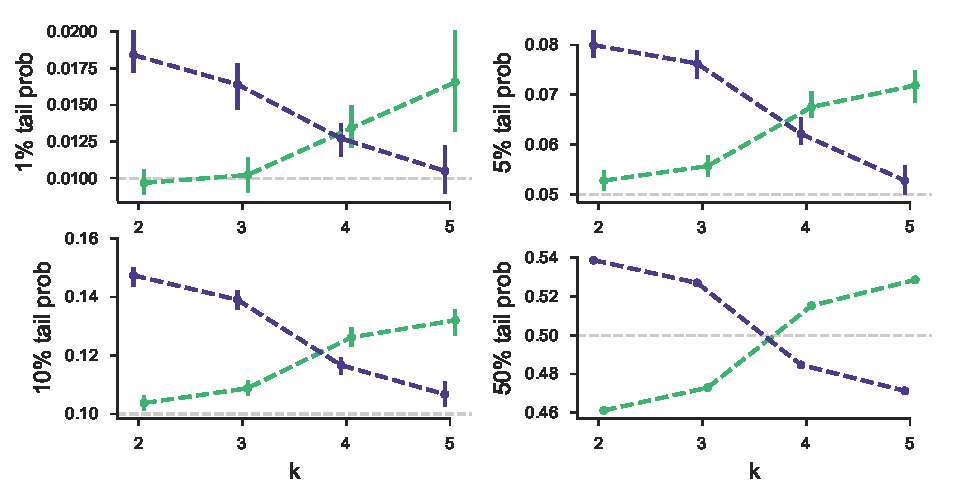
\includegraphics[]{figures/barghi-tailprobs-panels.pdf}

  \caption{ }
  \label{suppfig:barghi-tailprobs-panels}
\end{figure}





\end{document}
